% !TeX root = ../../../master.tex

\subsection{Ordnerstruktur}
\label{ssec:Ordnerstruktur}

Wie bereits in den Kapiteln~\vref{ssec:React} und \vref{ssec:AufbauReact} dargelegt, werden für den Aufbau der Anwendung verschiedene Komponenten benötigt.

Abbildung~\myRefGeneral{fig:OrdnerstrukturVSCode} zeigt einen Ausschnitt der Ordnerstruktur in der \ac{IDE} \emph{Visual Studio Code (VS Code)}.\footnote{\url{https://code.visualstudio.com}}
Exemplarisch werden kurz die \emph{Card-Komponente} sowie die \emph{Admin-Komponente} erläutert, deren Ergebnisse später \ua in dem Kapitel \vref{ssec:Administrationsbereich} aufgezeigt werden.

Für jede Komponente wird \ua zur besseren Übersicht \emph{(separation of code)} in der VS Code ein eigener Ordner angelegt, der die Komponente selbst (wie \zb \jinline|Admin| oder \jinline|Card|) sowie die Kind-Komponenten (wie \zb \jinline|CreateUserCard|) enthält.
Des Weiteren wird eine spezifische \emph{\acs{CSS}}-Datei je Komponente angelegt, mit der Anpassungen am späteren Aussehen durchgeführt werden können.
Dies könnte \zb die Farbe in \enquote{DHBW-rot} sein.
Damit einhergehend kann ein differenzierter und übersichtlicher Code erzeugt werden \emph{(separation of concerns)}.

Wie bereits beschrieben kann eine Komponente mehrere Kind-Komponenten und diese ebenfalls wieder mehrere Kind-Komponenten enthalten.
So fungiert die Klasse \jinline|Card| \ua als Kind-Komponente der Komponente \jinline|CreateUserCard|, \jinline|RegisterKeyCard| und \jinline|ShowUsersCard|.

\begin{figure}[!htb]
	\centering
	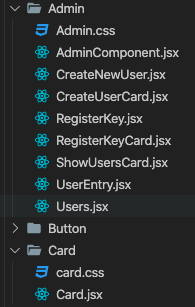
\includegraphics[height=0.4\textwidth, keepaspectratio]{img/client/ordnerStruktur.png}
	\captionsetup{justification=centering, format=plain}
	\caption[Ordnerstruktur des Front-Ends]{Ordnerstruktur des Front-Ends \\ \quelleScreenshot}
	\label{fig:OrdnerstrukturVSCode}
\end{figure}
